\documentclass[sigconf,nonacm]{acmart}

% Remove ACM copyright and conference info
\settopmatter{printacmref=false}
\renewcommand\footnotetextcopyrightpermission[1]{}
\pagestyle{plain}

\usepackage{booktabs}
\usepackage{graphicx}
\usepackage{multirow}
\usepackage{adjustbox}
\usepackage{microtype}  % Better text justification
\usepackage{hyphenat}   % Better hyphenation
\usepackage{ragged2e}   % Better ragged text
\usepackage[table]{xcolor}  % For row coloring
\usepackage{colortbl}       % For table colors

% Allow better line breaking
\sloppy
\hyphenpenalty=5000
\tolerance=1000

\begin{document}

\title{Prompt Enrichment Evaluation for News Classification with Open Source LLMs}

\author{V. Adrian Castillo}
\email{vacl2@byu.edu}
\affiliation{%
  \institution{Brigham Young University}
  \city{Provo}
  \state{UT}
}

\begin{abstract}
Large language models have demonstrated effectiveness in news classification through prompting. Drawing inspiration from enriched category representations in news recommendation systems, this study systematically evaluates whether detailed category descriptions improve news classification compared to label-only prompts. We assess four prompting techniques (zero-shot, few-shot-3, few-shot-5, chain-of-thought) across three open-source decoder-only LLMs (Gemma3:12b, Llama3.2:1b, GPT-OSS:20b) on three benchmark news datasets (AG News, BBC News, 20 Newsgroups). We find that enrichment effectiveness is highly technique dependent. Chain-of-thought prompting benefits substantially from enrichment, while few-shot techniques show neutral to negative effects. However, even enriched chain-of-thought underperforms baseline few-shot approaches by substantial margins, demonstrating that enrichment cannot compensate for technique-task misalignment. Model robustness varies significantly, with Gemma3:12b maintaining stable performance while GPT-OSS:20b exhibits catastrophic parse failure rates exceeding 80\% on complex datasets despite its larger parameter count.
\end{abstract}

\maketitle

\section{Introduction}

News classification represents a fundamental task in natural language processing with applications in content curation, automated journalism, and information filtering systems. The exponential growth of online news content necessitates effective automated categorization methods. Large language models have enabled prompt-based news classification approaches that achieve competitive performance without task-specific fine-tuning, yet optimal prompting strategies for news categorization remain an active research question.

This study systematically evaluates semantic category enrichment for news classification across two research questions. First, we assess whether enriched descriptions improve news classification performance. Second, we examine how enrichment effectiveness varies across prompting techniques representing different paradigms: instruction-only (zero-shot), demonstration-based (few-shot with three and five examples), and reasoning-based (chain-of-thought) approaches.

Results demonstrate that enrichment effectiveness depends critically on prompting technique rather than applying uniformly across news classification scenarios. Chain-of-thought prompting gains substantially from enrichment across all performance metrics, while few-shot techniques degrade. These patterns reveal that enrichment provides semantic anchors supporting structured reasoning but introduces redundancy when labeled news examples already demonstrate category boundaries. Critically, enriched chain-of-thought remains inferior to simpler approaches in absolute terms despite substantial relative gains, establishing that semantic enrichment cannot compensate for fundamental technique-task misalignment in news classification.

Model architecture significantly influences reliability through parse failure rates rather than through parameter count alone. The 12-billion-parameter Gemma3 model maintains stable performance with controlled parse failures, while the 20-billion-parameter GPT-OSS model exhibits catastrophically high failure rates that overwhelm potential accuracy gains. This finding demonstrates that instruction-tuning quality and output formatting training matter more for practical deployment than raw model scale, aligning with recent findings on the importance of instruction tuning for model reliability~\cite{zhang2023instruction, gretz2023zero}.

\section{Related Work}

Yada and Yamana~\cite{yada2024news} proposed automatically generating category descriptions for news recommendation using large language models, demonstrating that enriched categories improved recommendation AUC by up to 5.8\% compared to label-only approaches. Their method generated informative keywords for news categories, then incorporated these descriptions into neural recommendation architectures. Zhang et al.~\cite{zhang2024teleclass} introduced TELEClass for weakly-supervised hierarchical text classification, showing that LLM-generated keywords consolidate category meanings and benefit fine-grained class distinction. However, these studies focused on encoder-based or encoder-decoder architectures, leaving decoder-only models in zero-shot and few-shot news classification contexts unexplored.

Research on prompting techniques has established distinct paradigms. Few-shot prompting has proven effective for classification, with Brown et al.~\cite{brown2020language} demonstrating that labeled examples within prompts enable competitive performance. Chain-of-thought prompting~\cite{wei2022chain} significantly improves performance on arithmetic and symbolic reasoning tasks, with gains primarily in large models exceeding 100 billion parameters. Importantly, Wei et al. noted that classification tasks may not benefit equivalently, observing that ``for classification, many exemplars'' provide more effective supervision than explicit reasoning steps. Recent research emphasizes that model performance depends not only on parameter count but also on instruction-tuning quality, with smaller well-tuned models often outperforming larger models with poor tuning~\cite{zhang2023instruction, gretz2023zero}. Sun et al.~\cite{sun2023text} explored text classification via large language models, demonstrating that progressive reasoning strategies can improve performance when appropriately designed for task structure.

\section{Methodology}

\subsection{Category Description Enrichment}

Our core contribution adapts semantic enrichment from news recommendation systems to prompt-based news classification. Traditional prompts specify categories as simple labels (e.g., ``Categories: Sports, Business, Technology, World''). We propose enriched descriptions providing semantic context (e.g., ``Categories: Sports (athletic competitions, games, teams, players, championships, tournaments, Olympics, leagues), Business (companies, markets, economy, finance, stocks, trading, corporations, revenue) ...'').

The same enriched descriptions were used consistently across all experiments. Complete enrichment descriptions for all datasets are provided in Appendix~\ref{app:enriched}.

\subsection{Datasets}

We evaluate enrichment across three benchmark news classification datasets with varying difficulty levels. Table~\ref{tab:datasets} summarizes dataset characteristics.

\begin{table}[h]
\centering
\small
\begin{tabular}{@{}p{1.8cm}p{2.2cm}p{1.5cm}p{1.2cm}@{}}
\toprule
\textbf{Dataset} & \textbf{Categories} & \textbf{Size} & \textbf{Domain} \\ 
\midrule
AG News & 4 (Sports, Business, Sci/Tech, World) & 120K train / 7.6K test & News articles \\
\midrule
BBC News & 5 (Business, Entertain\-ment, Politics, Sport, Tech) & $\sim$2,225 articles & News articles \\
\midrule
20 News\-groups & 20 topics & $\sim$18K documents & Discussion forums \\
\bottomrule
\end{tabular}
\caption{Dataset Characteristics}
\label{tab:datasets}
\end{table}

AG News provides a baseline for coarse-grained classification with clear semantic boundaries. BBC News introduces finer distinctions with potential overlap between Business and Technology categories. 20 Newsgroups presents the greatest challenge, requiring models to distinguish between closely related topics spanning technical, scientific, recreational, and political domains.

\subsection{Models}

We evaluate three recent open-source decoder-only LLMs representing different parameter scales and instruction-tuning approaches: Gemma3:12b (12 billion parameters), Llama3.2:1b (1 billion parameters), and GPT-OSS:20b (20 billion parameters). This selection enables comparison of how model characteristics interact with enrichment effectiveness, testing whether parameter count predicts enrichment benefits or output reliability. All models were released between 2024 and 2025, ensuring evaluation on contemporary architectures.

\subsection{Prompting Techniques}

We evaluate four prompting techniques, each in baseline and enriched variants, representing distinct paradigms for in-context learning. Zero-shot prompting provides only task instructions and category labels without examples, testing whether models can leverage enriched descriptions as the sole source of category information. This technique isolates the effect of semantic descriptions independent of demonstration-based learning.

Few-shot prompting includes labeled news examples before the target instance, enabling models to learn category boundaries from demonstrations. We test 3-shot and 5-shot variants based on prior findings showing saturation beyond 3-5 examples for classification tasks~\cite{brown2020language} and practical context length constraints. Examples were selected through stratified random sampling from training data, ensuring balanced representation across categories. The same example sets remain fixed across all test instances within each dataset-model combination, eliminating variability from example selection.

For enriched few-shot variants, both semantic descriptions and labeled examples are provided, testing whether enrichment provides additional benefit beyond pattern recognition from examples. This design enables assessment of whether enrichment introduces redundancy or complementary information.

Chain-of-thought prompting encourages explicit reasoning through a three-step structure: (1) identify the main topic and key themes, (2) match themes to category descriptions, (3) provide final answer. Wei et al.~\cite{wei2022chain} demonstrated that CoT substantially improves arithmetic and symbolic reasoning tasks requiring multi-step inference, though they noted classification may not benefit equivalently since ``for classification, many exemplars'' typically provide more effective supervision than explicit reasoning. Our CoT implementation tests whether semantic enrichment can enhance reasoning-based classification despite this documented limitation.

Each prompting technique was implemented with identical structural formatting, varying only in the presence/absence of category descriptions (baseline vs. enriched) and examples (zero-shot vs. few-shot). Complete prompt templates are provided in Appendix~\ref{app:prompts}.

\subsection{Experimental Setup}

All experiments were conducted using Ollama with consistent hardware configurations. We evaluated 300 stratified test samples per condition, selected to maintain proportional representation of all categories within each dataset. Temperature was set to zero for all experiments to ensure deterministic generation, eliminating sampling variability and enabling reliable comparison of enrichment effects. The same sample sets were used for all prompt variants within each dataset-model combination, ensuring that observed performance differences stem from prompting strategy rather than sample composition.

All prompts share identical structural formatting, varying only in category descriptions (label-only vs. enriched semantic descriptions). For few-shot prompts, we maintain consistent example ordering and formatting across baseline and enriched variants. This controlled design yields 72 experimental conditions: 3 models $\times$ 3 datasets $\times$ 8 technique variants (4 techniques $\times$ 2 enrichment conditions).

Performance evaluation uses four standard classification metrics computed for each experimental condition: accuracy, precision, recall, and F1 score. Parse failures were recorded separately when models produced outputs not conforming to the required single-category format, as these indicate practical reliability issues regardless of classification performance on successfully parsed outputs.

\section{Results}

We present results addressing our two research questions through comprehensive evaluation across models, datasets, and prompting techniques. Table~\ref{tab:results} presents complete results organized by model and technique, with performance metrics grouped by dataset.



\begin{table*}[t]
\centering
\small
\begin{adjustbox}{width=\textwidth}
\begin{tabular}{@{}llrrrrrrrrrrrr@{}}
\toprule
\textbf{Model} & \textbf{Technique} & \multicolumn{4}{c}{\textbf{AG News}} & \multicolumn{4}{c}{\textbf{BBC News}} & \multicolumn{4}{c}{\textbf{20 Newsgroups}} \\
\cmidrule(lr){3-6} \cmidrule(lr){7-10} \cmidrule(lr){11-14}
& & \textbf{Acc} & \textbf{Prec} & \textbf{Rec} & \textbf{F1} & \textbf{Acc} & \textbf{Prec} & \textbf{Rec} & \textbf{F1} & \textbf{Acc} & \textbf{Prec} & \textbf{Rec} & \textbf{F1} \\
\midrule
\multirow{8}{*}{Gemma3:12b} 
& Zero-shot & 83.7 & 86.9 & 83.7 & 83.0 & 93.0 & 93.9 & 92.1 & 92.6 & 54.7 & 72.3 & 53.6 & 55.8 \\
& \cellcolor{gray!10}Zero-shot (enriched) & \cellcolor{gray!10}84.7 & \cellcolor{gray!10}86.6 & \cellcolor{gray!10}84.7 & \cellcolor{gray!10}84.4 & \cellcolor{gray!10}95.3 & \cellcolor{gray!10}95.8 & \cellcolor{gray!10}94.9 & \cellcolor{gray!10}95.2 & \cellcolor{gray!10}60.0 & \cellcolor{gray!10}72.6 & \cellcolor{gray!10}58.8 & \cellcolor{gray!10}61.3 \\
& Few-shot-3 & 83.7 & 85.9 & 83.7 & 83.4 & 94.0 & 94.0 & 93.6 & 93.7 & 62.0 & 72.8 & 60.4 & 61.4 \\
& \cellcolor{gray!10}Few-shot-3 (enriched) & \cellcolor{gray!10}84.3 & \cellcolor{gray!10}86.1 & \cellcolor{gray!10}84.3 & \cellcolor{gray!10}84.1 & \cellcolor{gray!10}95.0 & \cellcolor{gray!10}95.4 & \cellcolor{gray!10}94.6 & \cellcolor{gray!10}94.8 & \cellcolor{gray!10}\textbf{66.0} & \cellcolor{gray!10}71.6 & \cellcolor{gray!10}\textbf{64.7} & \cellcolor{gray!10}\textbf{65.8} \\
& Few-shot-5 & 85.7 & 86.8 & 85.7 & 85.5 & \textbf{95.7} & 95.9 & 95.2 & \textbf{95.4} & 61.3 & 74.0 & 60.3 & 61.4 \\
& \cellcolor{gray!10}Few-shot-5 (enriched) & \cellcolor{gray!10}\textbf{86.3} & \cellcolor{gray!10}86.8 & \cellcolor{gray!10}\textbf{86.3} & \cellcolor{gray!10}\textbf{86.3} & \cellcolor{gray!10}\textbf{95.7} & \cellcolor{gray!10}95.8 & \cellcolor{gray!10}\textbf{95.3} & \cellcolor{gray!10}\textbf{95.4} & \cellcolor{gray!10}65.3 & \cellcolor{gray!10}69.0 & \cellcolor{gray!10}63.8 & \cellcolor{gray!10}65.1 \\
& Chain-of-thought & 45.3 & 82.9 & 45.3 & 36.9 & 52.0 & 74.7 & 48.8 & 46.6 & 30.7 & 69.5 & 29.8 & 38.1 \\
& \cellcolor{gray!10}CoT (enriched) & \cellcolor{gray!10}67.0 & \cellcolor{gray!10}80.8 & \cellcolor{gray!10}67.0 & \cellcolor{gray!10}66.4 & \cellcolor{gray!10}78.0 & \cellcolor{gray!10}84.3 & \cellcolor{gray!10}76.2 & \cellcolor{gray!10}76.3 & \cellcolor{gray!10}52.7 & \cellcolor{gray!10}71.0 & \cellcolor{gray!10}51.2 & \cellcolor{gray!10}57.0 \\
\midrule
\multirow{8}{*}{Llama3.2:1b} 
& Zero-shot & 51.7 & 63.6 & 51.7 & 60.5 & 59.0 & 84.4 & 56.6 & 54.1 & 7.3 & 26.8 & 7.4 & 14.3 \\
& \cellcolor{gray!10}Zero-shot (enriched) & \cellcolor{gray!10}50.0 & \cellcolor{gray!10}68.8 & \cellcolor{gray!10}50.0 & \cellcolor{gray!10}58.3 & \cellcolor{gray!10}31.0 & \cellcolor{gray!10}62.1 & \cellcolor{gray!10}31.4 & \cellcolor{gray!10}30.9 & \cellcolor{gray!10}10.7 & \cellcolor{gray!10}23.0 & \cellcolor{gray!10}10.7 & \cellcolor{gray!10}18.4 \\
& Few-shot-3 & 55.0 & 68.1 & 55.0 & 64.9 & 88.0 & 89.5 & 87.2 & 87.9 & 8.3 & 33.9 & 8.4 & 17.5 \\
& \cellcolor{gray!10}Few-shot-3 (enriched) & \cellcolor{gray!10}48.7 & \cellcolor{gray!10}68.4 & \cellcolor{gray!10}48.7 & \cellcolor{gray!10}57.6 & \cellcolor{gray!10}30.7 & \cellcolor{gray!10}74.3 & \cellcolor{gray!10}31.6 & \cellcolor{gray!10}38.1 & \cellcolor{gray!10}8.0 & \cellcolor{gray!10}26.2 & \cellcolor{gray!10}8.2 & \cellcolor{gray!10}17.8 \\
& Few-shot-5 & 60.0 & 71.8 & 60.0 & 71.7 & 84.3 & 87.9 & 83.0 & 83.4 & 6.3 & 12.7 & 6.6 & 10.2 \\
& \cellcolor{gray!10}Few-shot-5 (enriched) & \cellcolor{gray!10}54.0 & \cellcolor{gray!10}72.7 & \cellcolor{gray!10}54.0 & \cellcolor{gray!10}63.4 & \cellcolor{gray!10}38.0 & \cellcolor{gray!10}80.6 & \cellcolor{gray!10}39.5 & \cellcolor{gray!10}43.1 & \cellcolor{gray!10}9.3 & \cellcolor{gray!10}33.7 & \cellcolor{gray!10}10.0 & \cellcolor{gray!10}21.0 \\
& Chain-of-thought & 30.0 & 56.8 & 30.0 & 19.6 & 50.3 & 70.7 & 46.5 & 42.1 & 7.7 & 25.3 & 7.6 & 15.8 \\
& \cellcolor{gray!10}CoT (enriched) & \cellcolor{gray!10}36.0 & \cellcolor{gray!10}64.0 & \cellcolor{gray!10}36.0 & \cellcolor{gray!10}33.5 & \cellcolor{gray!10}56.3 & \cellcolor{gray!10}69.7 & \cellcolor{gray!10}54.7 & \cellcolor{gray!10}54.6 & \cellcolor{gray!10}13.7 & \cellcolor{gray!10}31.4 & \cellcolor{gray!10}13.7 & \cellcolor{gray!10}20.0 \\
\midrule
\multirow{8}{*}{GPT-OSS:20b} 
& Zero-shot & 61.7 & 92.0 & 61.7 & 71.9 & 86.3 & 97.1 & 85.1 & 89.9 & 18.3 & \textbf{98.7} & 17.5 & 39.6 \\
& \cellcolor{gray!10}Zero-shot (enriched) & \cellcolor{gray!10}65.0 & \cellcolor{gray!10}91.9 & \cellcolor{gray!10}65.0 & \cellcolor{gray!10}74.4 & \cellcolor{gray!10}83.7 & \cellcolor{gray!10}97.1 & \cellcolor{gray!10}82.2 & \cellcolor{gray!10}88.1 & \cellcolor{gray!10}20.3 & \cellcolor{gray!10}98.6 & \cellcolor{gray!10}19.4 & \cellcolor{gray!10}37.6 \\
& Few-shot-3 & 59.7 & 90.7 & 59.7 & 69.7 & 87.3 & 95.7 & 86.4 & 90.1 & 18.3 & 90.6 & 17.6 & 45.6 \\
& \cellcolor{gray!10}Few-shot-3 (enriched) & \cellcolor{gray!10}56.0 & \cellcolor{gray!10}92.6 & \cellcolor{gray!10}56.0 & \cellcolor{gray!10}66.7 & \cellcolor{gray!10}87.7 & \cellcolor{gray!10}\textbf{98.1} & \cellcolor{gray!10}86.3 & \cellcolor{gray!10}91.0 & \cellcolor{gray!10}21.3 & \cellcolor{gray!10}95.8 & \cellcolor{gray!10}20.6 & \cellcolor{gray!10}41.8 \\
& Few-shot-5 & 57.0 & 92.1 & 57.0 & 68.5 & 87.3 & 97.1 & 86.5 & 90.8 & 20.0 & 87.2 & 19.2 & 45.2 \\
& \cellcolor{gray!10}Few-shot-5 (enriched) & \cellcolor{gray!10}55.0 & \cellcolor{gray!10}90.0 & \cellcolor{gray!10}55.0 & \cellcolor{gray!10}65.5 & \cellcolor{gray!10}85.7 & \cellcolor{gray!10}97.1 & \cellcolor{gray!10}84.5 & \cellcolor{gray!10}89.9 & \cellcolor{gray!10}23.0 & \cellcolor{gray!10}97.8 & \cellcolor{gray!10}22.2 & \cellcolor{gray!10}40.1 \\
& Chain-of-thought & 59.7 & 92.4 & 59.7 & 70.0 & 82.3 & 97.3 & 80.8 & 86.8 & 14.3 & 92.3 & 13.7 & 34.8 \\
& \cellcolor{gray!10}CoT (enriched) & \cellcolor{gray!10}64.7 & \cellcolor{gray!10}\textbf{92.8} & \cellcolor{gray!10}64.7 & \cellcolor{gray!10}74.5 & \cellcolor{gray!10}82.0 & \cellcolor{gray!10}97.0 & \cellcolor{gray!10}80.2 & \cellcolor{gray!10}86.5 & \cellcolor{gray!10}14.7 & \cellcolor{gray!10}96.4 & \cellcolor{gray!10}14.1 & \cellcolor{gray!10}35.3 \\
\bottomrule
\end{tabular}
\end{adjustbox}
\caption{Performance Results Across All Models, Datasets, and Techniques}
\label{tab:results}
\end{table*}

\subsection{Enrichment Effects by Technique and Precision-Recall Patterns}

Enrichment effectiveness varies systematically by prompting paradigm, with critical differences emerging in precision-recall balance. Chain-of-thought prompting demonstrates the most substantial improvements from enrichment. For Gemma3:12b on AG News, enrichment increases F1 score by 29.5 points (36.9 to 66.4), with balanced improvements across precision (82.9\% to 80.8\%) and recall (45.3\% to 67.0\%). On BBC News, F1 improves by 29.7 points (46.6 to 76.3), with recall gains of 27.4 points. These patterns validate that reasoning-based prompts benefit from semantic grounding when models must explicitly articulate classification rationale.

However, baseline chain-of-thought exhibits severe precision-recall imbalance that enrichment only partially addresses. On 20 Newsgroups, baseline CoT achieves 69.5\% precision but only 29.8\% recall, resulting in just 38.1 F1. Enrichment improves recall to 51.2\% while maintaining 71.0\% precision, yielding 57.0 F1—a substantial relative improvement of 18.9 points, yet the technique remains overly conservative in category assignment.

Despite enrichment gains, chain-of-thought consistently underperforms few-shot approaches across all metrics. On AG News, enriched CoT achieves 67.0 F1 compared to few-shot-3's 83.4 F1—a gap of 16.4 points. On BBC News, the gap is 17.4 points (76.3 vs 93.7 F1). Few-shot methods maintain tight precision-recall coupling (within 2.2 points across all Gemma3:12b conditions), while CoT shows persistent imbalances exceeding 15 points even with enrichment.

Few-shot techniques show divergent enrichment effects across models and pronounced differences in precision-recall stability. Gemma3:12b demonstrates modest improvements or neutral effects, with few-shot-3 enrichment on 20 Newsgroups improving F1 by 4.4 points (61.4 to 65.8) through balanced gains in both precision and recall. The model maintains precision-recall differences under 3 points across all few-shot conditions, indicating robust classification behavior.

Llama3.2:1b exhibits catastrophic failures with enrichment, particularly on BBC News where few-shot-3 enrichment causes F1 to collapse from 87.9 to 38.1—a 49.8 point drop. Analysis reveals this stems from severe recall degradation (87.2\% to 31.6\%) while precision remains elevated (74.3\%), suggesting the smaller model becomes overwhelmed by semantic complexity and adopts an overly conservative strategy. On AG News, enriched few-shot-5 drops from 71.7 to 63.4 F1, with similar precision-recall imbalance patterns emerging.

GPT-OSS:20b shows minimal enrichment effects across few-shot variants, with changes typically under 3 F1 points. However, the model exhibits an extreme precision-recall imbalance across all conditions. On 20 Newsgroups, the model achieves 90.6\% precision but only 17.6\% recall with few-shot-3, resulting in 45.6 F1 despite the high precision. This pattern indicates a conservative prediction strategy where the model only assigns categories when extremely confident, severely limiting practical utility by leaving most instances effectively unclassified or misclassified into a narrow subset of high-confidence categories.

\subsection{Model Architecture, Reliability, and Parse Failures}

Model performance reveals that parameter count alone does not predict classification effectiveness or reliability. Parse failure rates provide a critical reliability dimension that profoundly impacts practical deployment. Figure~\ref{fig:parse_failures} presents failure rates by model and dataset.

\begin{figure}[h]
    \centering
    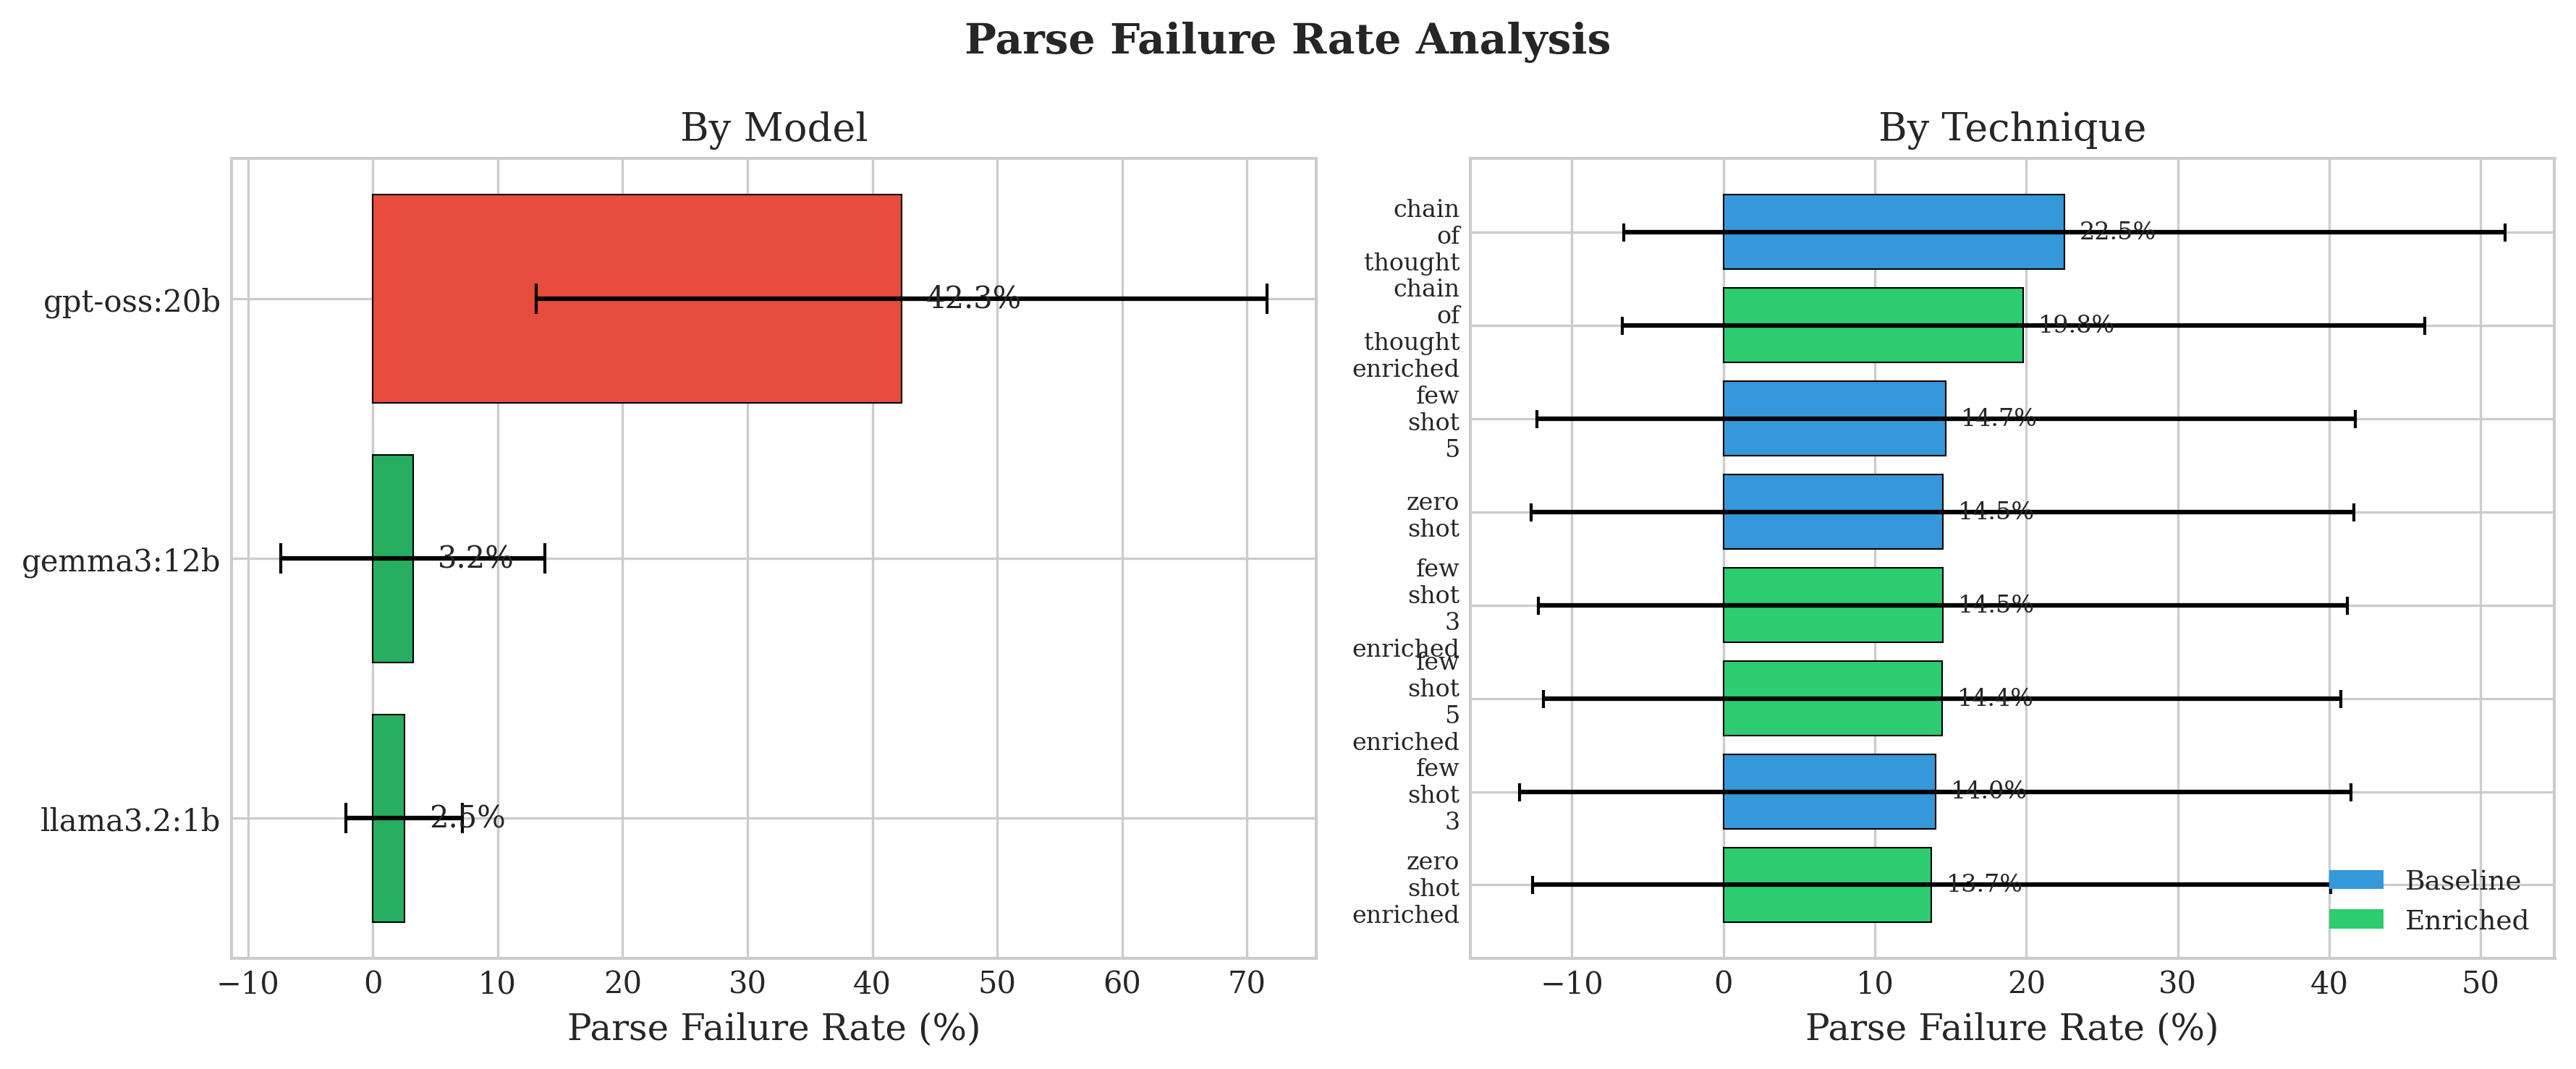
\includegraphics[width=\linewidth]{fig3_parse_failure_analysis.png}
    \caption{Parse failure rates by model and dataset, revealing that GPT-OSS:20b exhibits catastrophically high failure rates on 20 Newsgroups (exceeding 80\%), while Gemma3:12b and Llama3.2:1b maintain stable rates below 5\% across datasets.}
    \label{fig:parse_failures}
\end{figure}

GPT-OSS:20b exhibits catastrophically high parse failure rates on 20 Newsgroups, exceeding 80\% across most conditions. These failures occur when the model produces improperly formatted output—generating explanatory text, multiple categories, or refusing to classify rather than providing single category predictions. Combined with the model's extreme precision-recall imbalance, these parse failures render the 20-billion-parameter model essentially unusable for complex classification tasks despite its parameter advantage. On simpler datasets, GPT-OSS maintains lower failure rates (under 15\%), but the conservative prediction strategy persists.

Gemma3:12b and Llama3.2:1b maintain parse failure rates below 5\% across all datasets, demonstrating robust output formatting regardless of dataset complexity. This stability indicates superior instruction-following and output constraint adherence, validating that effective instruction tuning matters more than parameter scale for reliable production deployment.

Beyond parse reliability, Gemma3:12b demonstrates the most consistent classification performance. On BBC News with few-shot-5, the model achieves balanced metrics: 95.7\% precision, 95.2\% recall, and 95.4 F1. On the challenging 20 Newsgroups dataset, Gemma3 maintains this balance with 74.0\% precision and 60.3\% recall, achieving 61.4 F1—substantially outperforming both the smaller Llama3.2:1b (10.2 F1) and larger GPT-OSS:20b (45.2 F1) despite their 1 billion and 20 billion parameter counts respectively.

Figure~\ref{fig:model_profiles} presents radar charts comparing model performance profiles across all metrics, illustrating these architectural differences.

\begin{figure}[h]
    \centering
    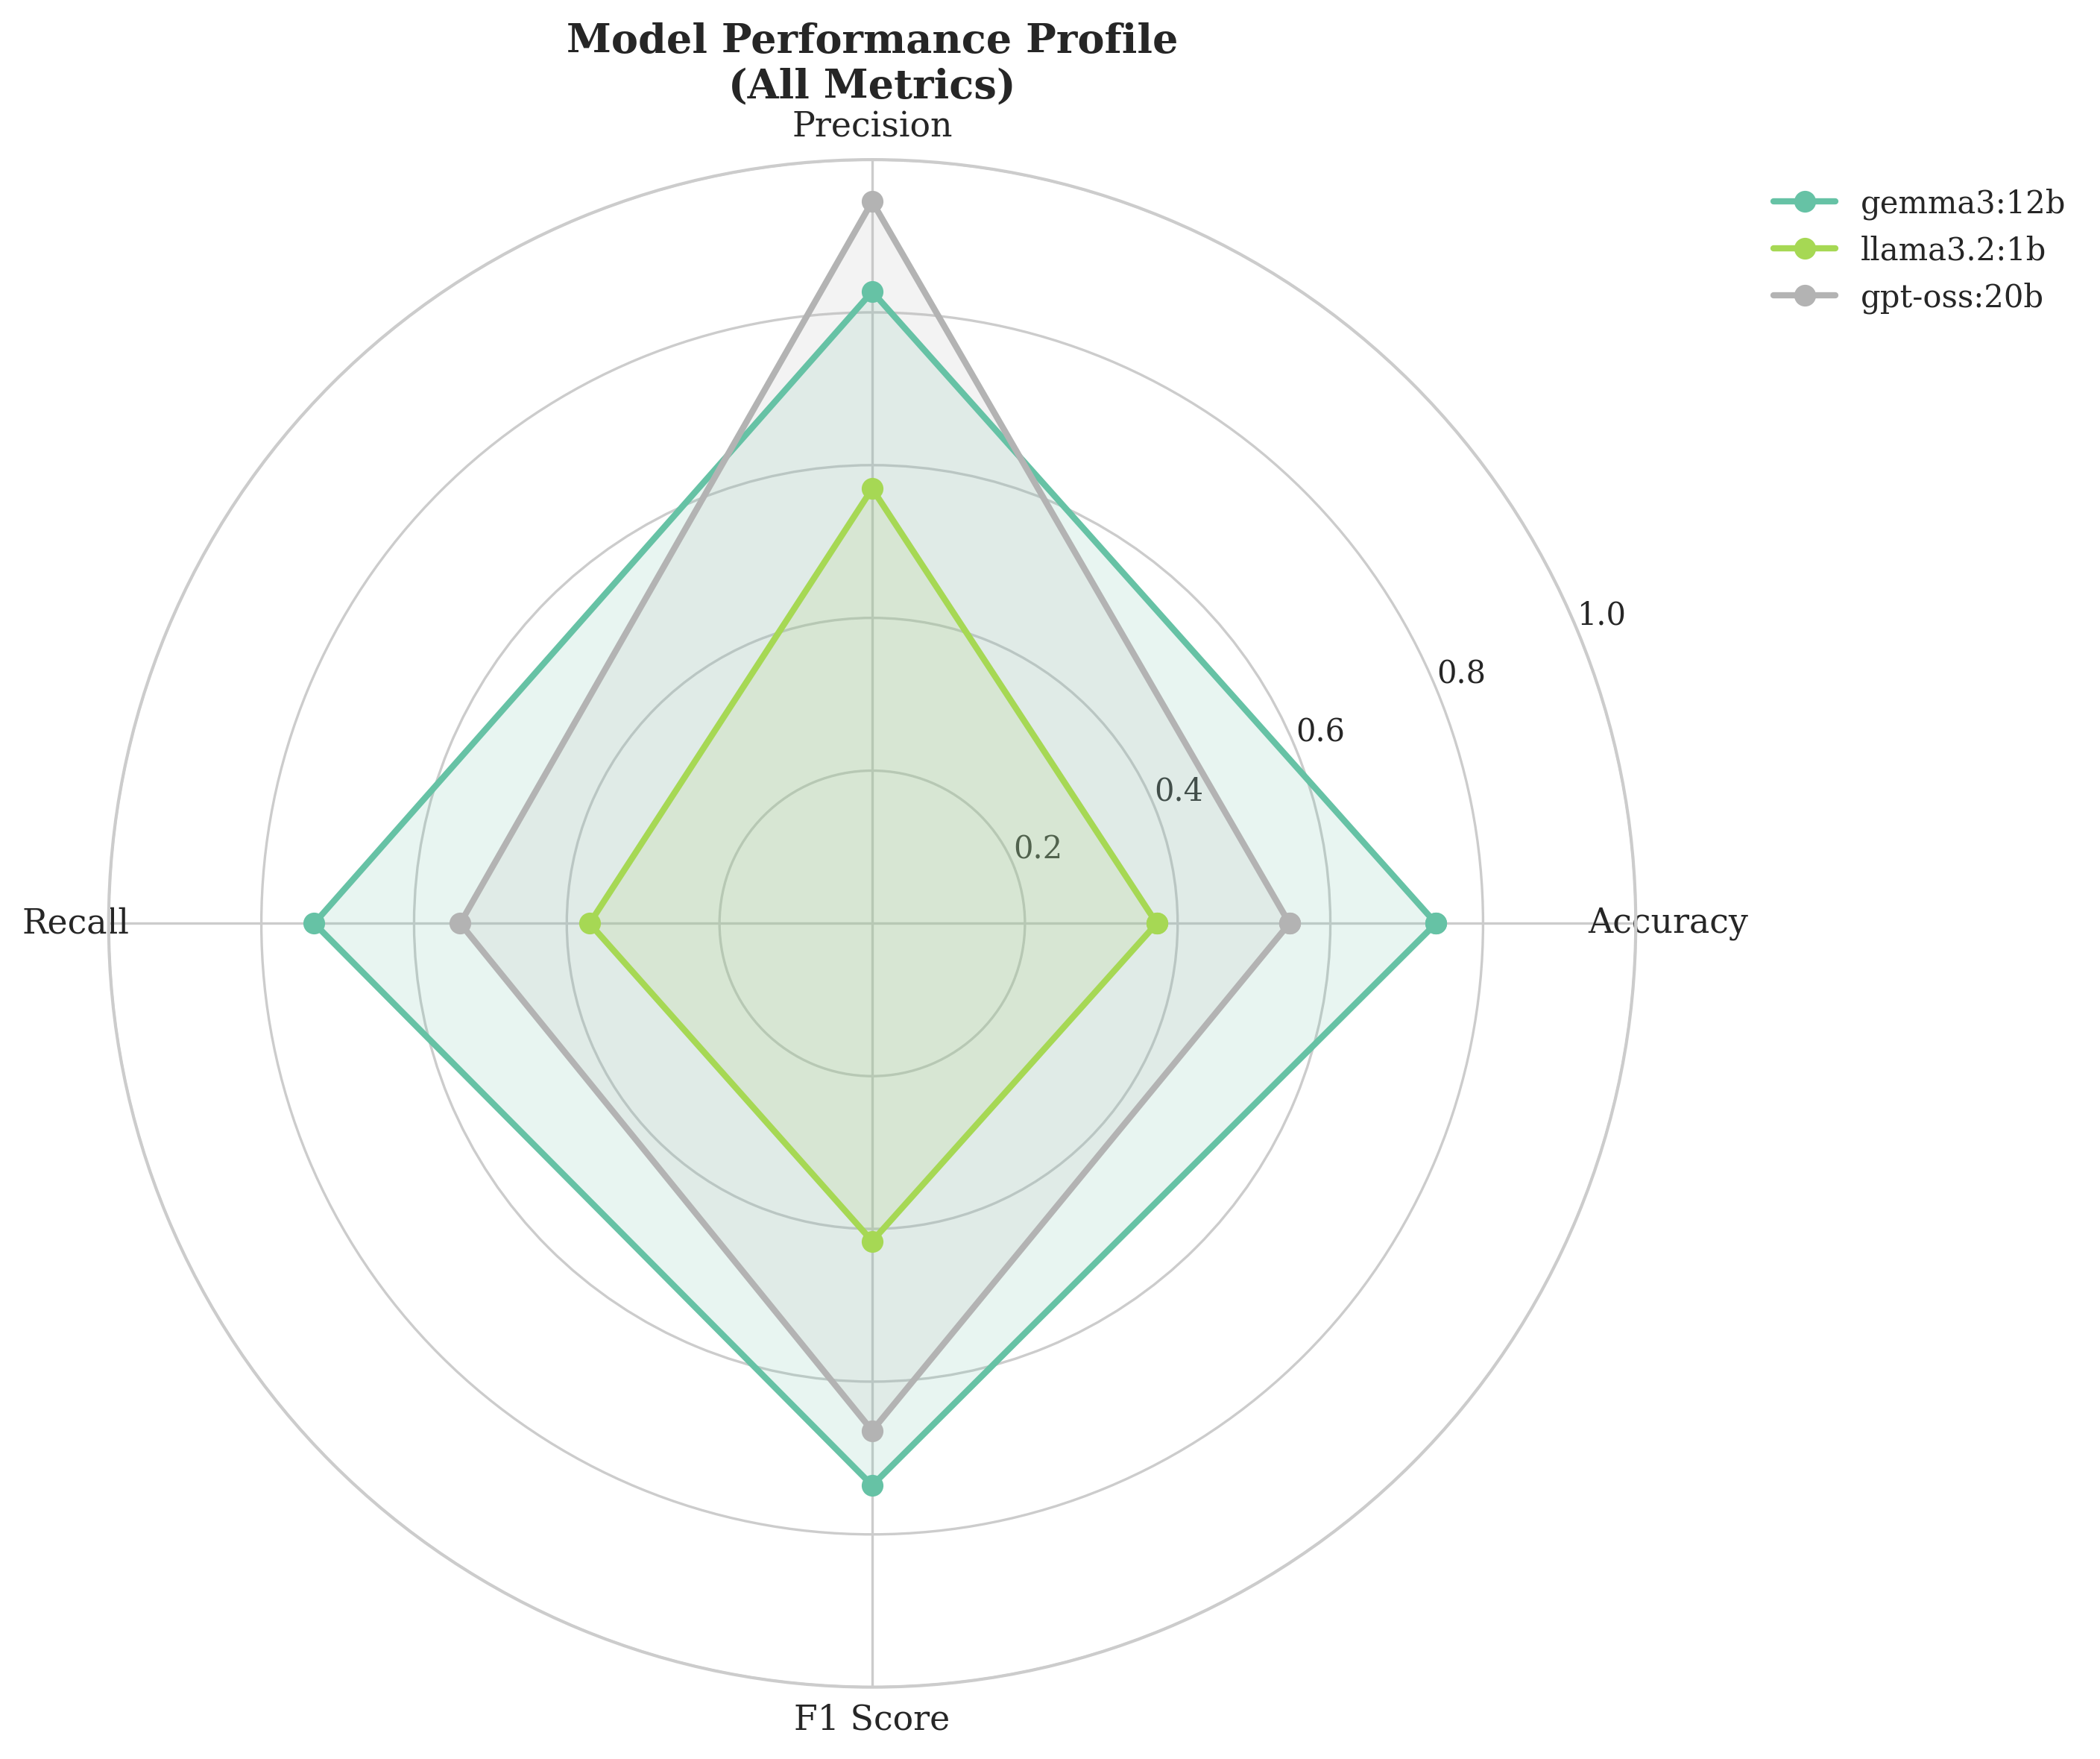
\includegraphics[width=\linewidth]{fig2_model_radar.png}
    \caption{Model performance profiles across accuracy, precision, recall, and F1 score, illustrating Gemma3:12b's balanced performance, GPT-OSS:20b's high-precision but low-recall pattern, and Llama3.2:1b's overall lower capabilities with high variability.}
    \label{fig:model_profiles}
\end{figure}

Llama3.2:1b shows unstable performance across metrics and high enrichment sensitivity. The model achieves competitive performance on simpler datasets without enrichment (88.0 F1 on BBC News with few-shot-3) but catastrophically fails when enrichment is applied to the same configuration (38.1 F1). This 49.9 point drop, driven by recall collapse from 87.2\% to 31.6\%, indicates insufficient model capacity to integrate complex semantic information with classification tasks.

\subsection{Dataset Complexity and Enrichment Interactions}

Dataset characteristics influence both absolute performance and enrichment sensitivity through ceiling effects and semantic disambiguation requirements. BBC News, with five well-separated categories, exhibits ceiling effects where baseline few-shot performance approaches optimal levels. Gemma3:12b achieves 93.7 F1 with few-shot-3 baseline, with balanced precision (94.0\%) and recall (93.6\%). Enrichment provides only 1.1 F1 point improvement to 94.8, suggesting diminishing returns when category boundaries are already well-defined through examples.

AG News, with four categories but greater semantic overlap, shows intermediate enrichment sensitivity. Business and Sci/Tech categories share vocabulary around companies and products, while World news overlaps with Business on economic themes. Few-shot enrichment provides modest F1 improvements for Gemma3:12b (0.7 points for few-shot-3, 0.8 points for few-shot-5), with enrichment helping disambiguate boundary cases through explicit semantic features.

20 Newsgroups presents maximum complexity with 20 fine-grained categories including multiple related groups (five comp.* categories, four talk.* categories, three sci.* categories). Here, enrichment shows substantial benefits for few-shot approaches. Gemma3:12b with few-shot-3 improves from 61.4 to 65.8 F1 with enrichment—a 4.4 point gain driven by balanced improvements in precision (72.8\% to 71.6\%) and recall (60.4\% to 64.7\%). The 4.3 point recall improvement indicates that semantic descriptions help models distinguish between related categories by providing explicit differentiating features.

Zero-shot prompting shows consistent enrichment benefits across all datasets and models, though absolute performance remains lower than few-shot approaches. Gemma3:12b gains 1.4 F1 points on AG News (83.0 to 84.4), 2.6 points on BBC News (92.6 to 95.2), and 5.5 points on 20 Newsgroups (55.8 to 61.3). These gains reflect enrichment's value when no examples are provided—semantic descriptions serve as the primary information source for category discrimination.

\subsection{Metric Variance and Technique Stability}

Performance variance across datasets reveals fundamental differences in technique stability. Figure~\ref{fig:metric_dist} illustrates metric distributions across prompting techniques for Gemma3:12b.

\begin{figure}[h]
    \centering
    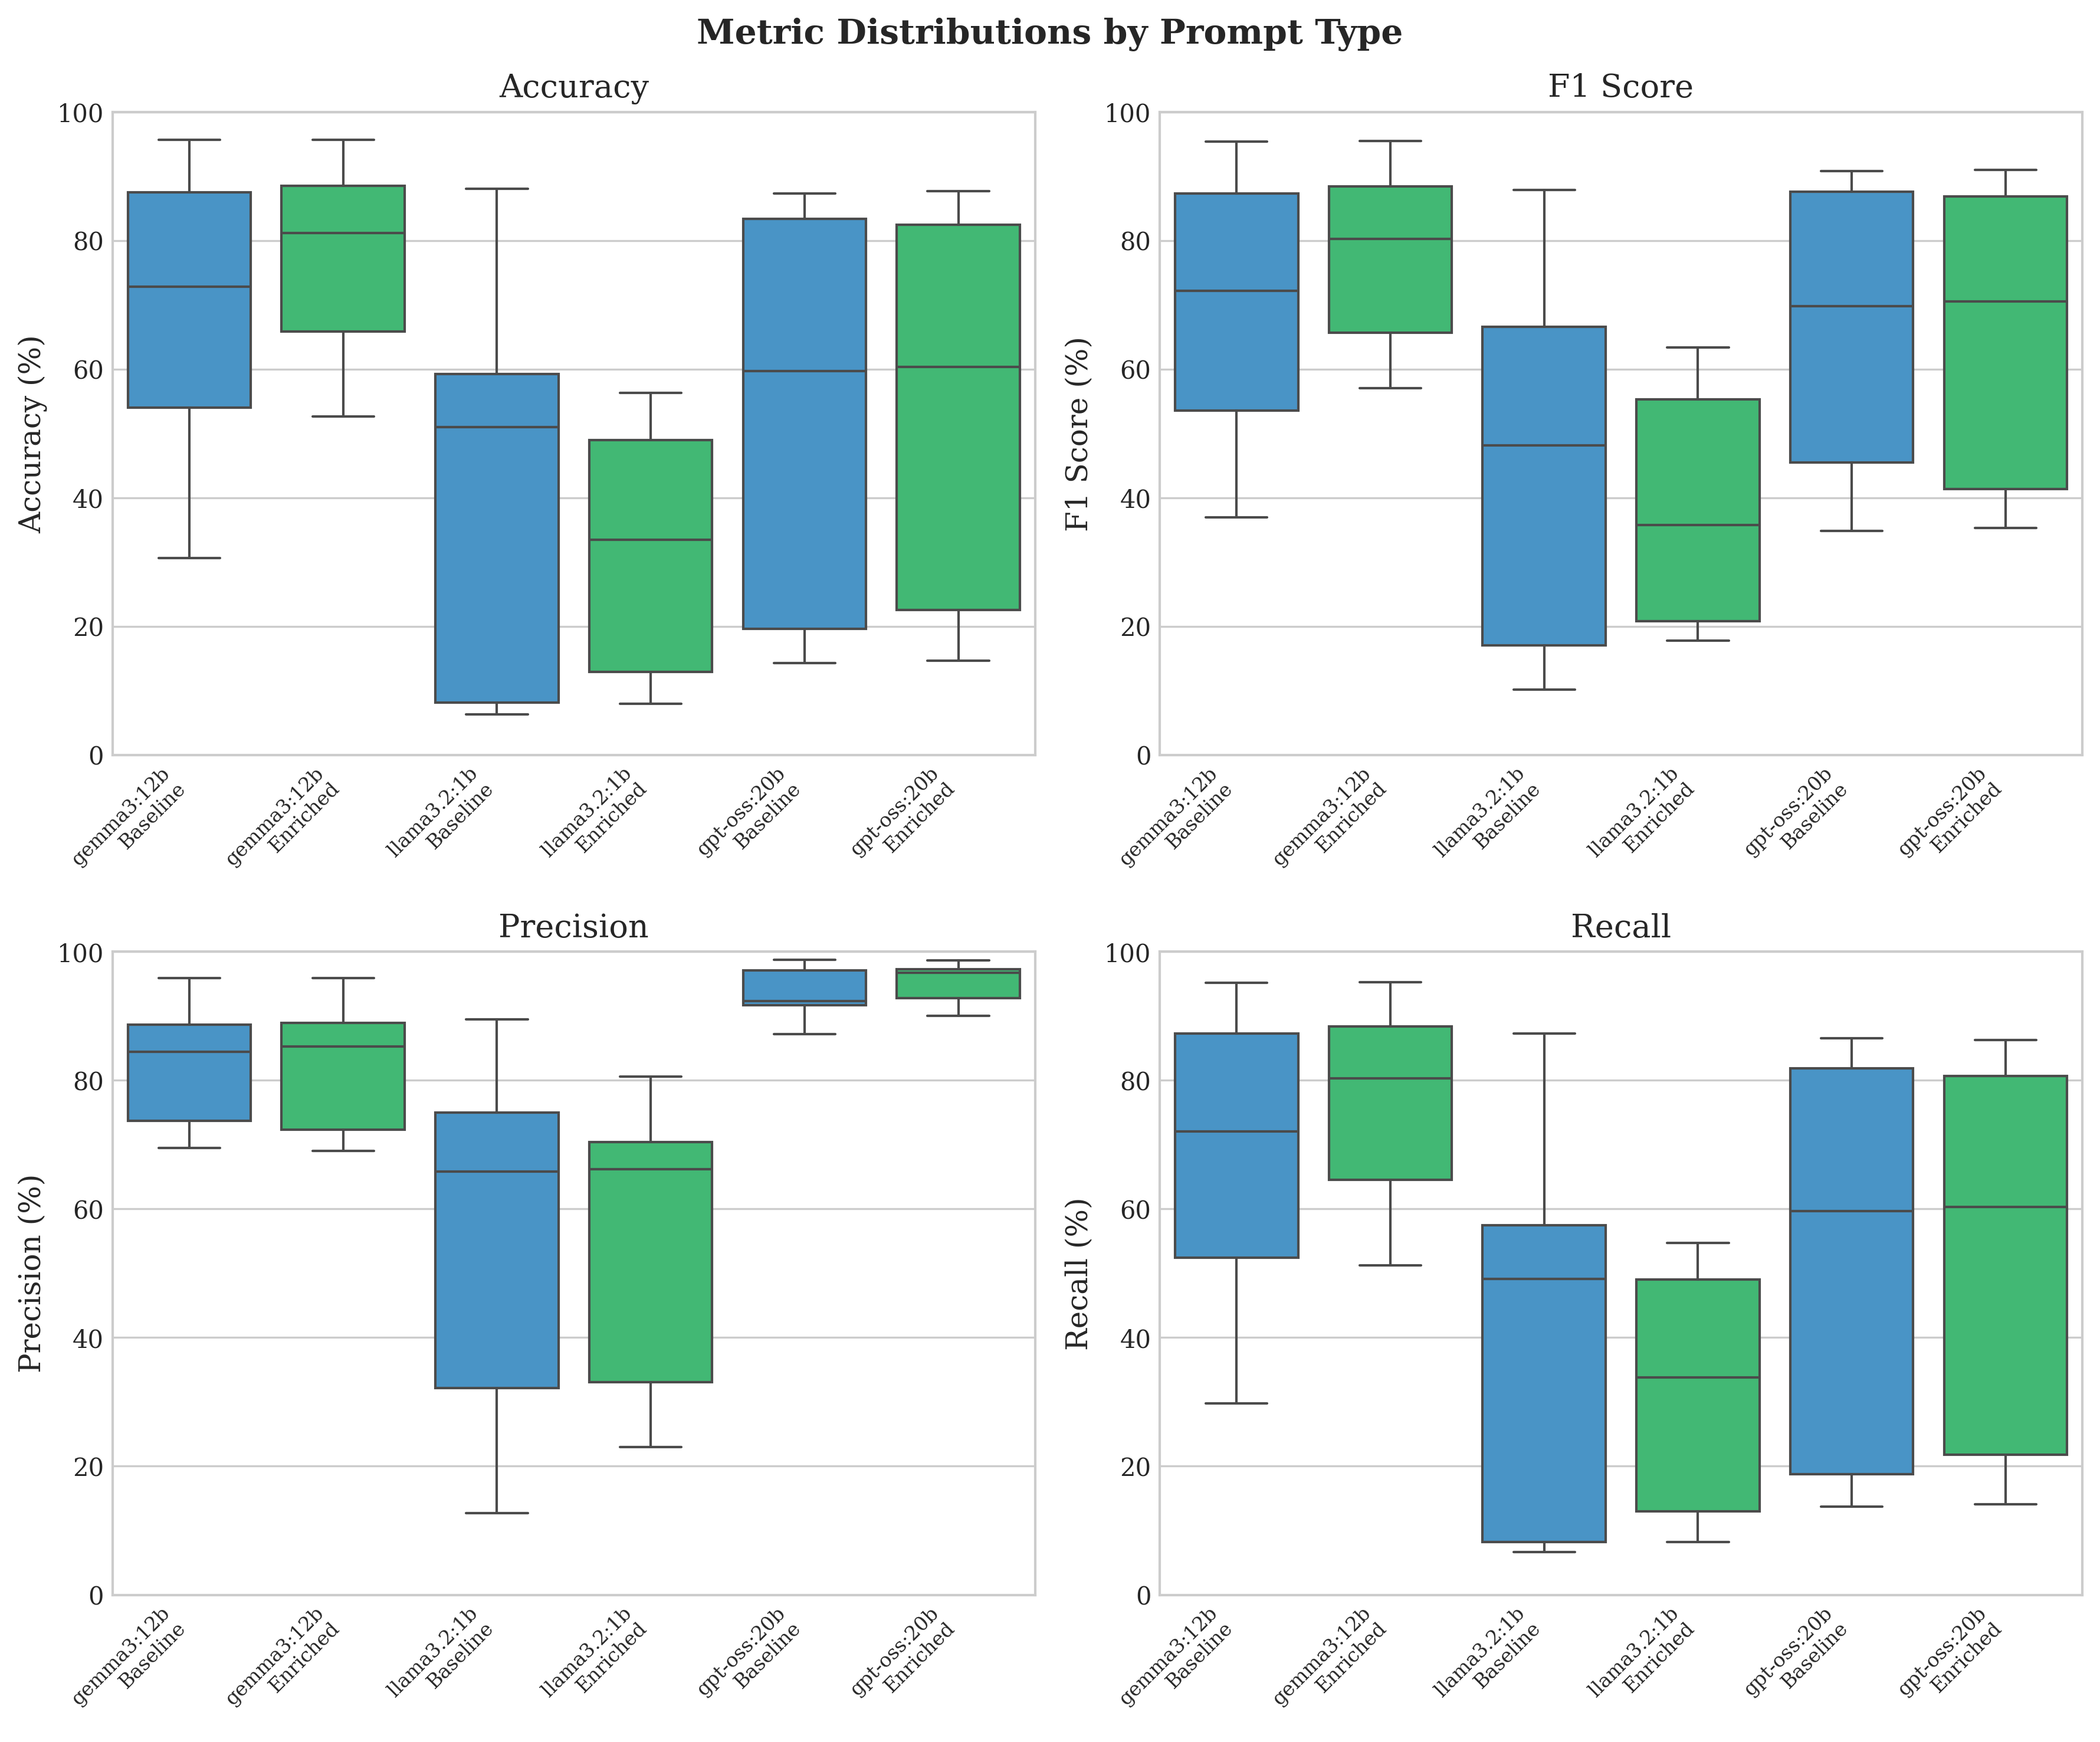
\includegraphics[width=\linewidth]{fig8_metric_distributions.png}
    \caption{Metric distributions across prompting techniques for Gemma3:12b, showing that few-shot methods maintain tight, high-performance distributions across accuracy, precision, recall, and F1 score, while chain-of-thought exhibits high variance and lower central performance despite enrichment gains.}
    \label{fig:metric_dist}
\end{figure}

Few-shot methods demonstrate remarkable consistency, with F1 standard deviations below 5 points across datasets. Precision and recall remain tightly coupled, with differences typically under 2 points. This stability indicates that labeled examples provide robust category boundary information regardless of dataset complexity.

Chain-of-thought methods show substantially higher variance, particularly in recall (standard deviation of 15.2 points across datasets compared to 3.1 for few-shot). On 20 Newsgroups, baseline CoT achieves 69.5\% precision but only 29.8\% recall—a 39.7 point gap. Enrichment reduces this imbalance to 19.8 points (71.0\% precision, 51.2\% recall) but cannot eliminate the fundamental precision-recall divergence. The persistent gap suggests CoT prompting encourages conservative behavior where models correctly classify instances they process but fail to confidently assign many articles to categories.

\section{Discussion}

Our results establish that enrichment effectiveness is highly technique-dependent and cannot compensate for fundamental technique-task misalignment. Chain-of-thought benefits substantially from enrichment through improved recall while maintaining high precision, yet consistently underperforms few-shot approaches across all metrics and datasets. The precision-recall imbalance in CoT—even with enrichment—reveals that explicit reasoning steps misalign with news classification's pattern-recognition nature. Few-shot methods with label-only descriptions maintain balanced precision-recall profiles and superior F1 scores, demonstrating the strongest performance for this task domain.

Model architecture analysis reveals instruction-tuning quality matters more than parameter count. Gemma3:12b's balanced metrics and sub-5\% parse failure rates demonstrate production readiness, while GPT-OSS:20b's 80\%+ parse failures on complex datasets render it impractical despite 20 billion parameters. This finding aligns with recent work emphasizing instruction tuning's critical role in model reliability~\cite{zhang2023instruction, gretz2023zero}.

For practitioners designing news classification systems, few-shot prompting with label-only descriptions achieves the strongest performance across precision, recall, and F1 score. Enrichment introduces redundancy when labeled examples already demonstrate category boundaries. Model selection should prioritize balanced precision-recall profiles and low parse failure rates over parameter count alone.

\section{Conclusions}

This study systematically evaluated whether enriched category descriptions improve news classification compared to label-only prompts. Results demonstrate that enrichment effectiveness is highly technique-dependent, with substantial benefits for reasoning-based approaches but neutral to negative effects for demonstration-based techniques.

Chain-of-thought prompting shows the largest improvement from enrichment across all performance metrics, yet even enriched chain-of-thought substantially underperforms baseline few-shot approaches. This establishes that semantic enrichment cannot compensate for fundamental technique-task misalignment in news classification. Few-shot prompting with label-only descriptions demonstrates the strongest performance across precision, recall, and F1 score without requiring enrichment overhead.

Model architecture analysis reveals that instruction-tuning quality and architectural design matter more than parameter count. The 12-billion-parameter Gemma3 maintains balanced performance across all metrics with stable output formatting, while the 20-billion-parameter GPT-OSS exhibits high precision but lower recall, and catastrophic parse failure rates exceeding 80\% on complex datasets.

Our findings establish that enrichment benefits depend critically on the alignment between prompting technique and task demands. When labeled examples effectively demonstrate category boundaries, enrichment introduces redundancy rather than clarity.

\bibliographystyle{ACM-Reference-Format}
\begin{thebibliography}{7}

\bibitem{zhang2023instruction}
Shengyu Zhang, Linfeng Dong, Xiaoya Li, Sen Zhang, Xiaofei Sun, Shuhe Wang, Jiwei Li, Runyi Hu, Tianwei Zhang, Fei Wu, and Guoyin Wang. 2023.
\newblock Instruction Tuning for Large Language Models: A Survey.
\newblock {\em arXiv preprint arXiv:2308.10792}.

\bibitem{gretz2023zero}
Shai Gretz, Alon Halfon, Ilya Shnayderman, Orith Toledo-Ronen, Artem Spector, Lena Dankin, Yannis Katsis, Ofir Arviv, Yoav Katz, Noam Slonim, and Liat Ein-Dor. 2023.
\newblock Zero-shot Topical Text Classification with LLMs - an Experimental Study.
\newblock In {\em Findings of the Association for Computational Linguistics: EMNLP 2023}, pages 9647--9676, Singapore. Association for Computational Linguistics.

\bibitem{yada2024news}
Yuki Yada and Hayato Yamana. 2024.
\newblock News Recommendation with Category Description by a Large Language Model.
\newblock {\em arXiv preprint arXiv:2405.13007}.

\bibitem{zhang2024teleclass}
Yunyi Zhang, Ruozhen Yang, Xueqiang Xu, Rui Li, Jinfeng Xiao, Jiaming Shen, and Jiawei Han. 2024.
\newblock TELEClass: Taxonomy Enrichment and LLM-Enhanced Hierarchical Text Classification with Minimal Supervision.
\newblock {\em arXiv preprint arXiv:2403.00165}.

\bibitem{brown2020language}
Tom Brown, Benjamin Mann, Nick Ryder, Melanie Subbiah, Jared D. Kaplan, Prafulla Dhariwal, Arvind Neelakantan, Pranav Shyam, Girish Sastry, Amanda Askell, Sandhini Agarwal, Ariel Herbert-Voss, Gretchen Krueger, Tom Henighan, Rewon Child, Aditya Ramesh, Daniel Ziegler, Jeffrey Wu, Clemens Winter, Chris Hesse, Mark Chen, Eric Sigler, Mateusz Litwin, Scott Gray, Benjamin Chess, Jack Clark, Christopher Berner, Sam McCandlish, Alec Radford, Ilya Sutskever, and Dario Amodei. 2020.
\newblock Language Models are Few-Shot Learners.
\newblock In {\em Proceedings of the 34th International Conference on Neural Information Processing Systems (NeurIPS 2020)}, pages 1877--1901.

\bibitem{wei2022chain}
Jason Wei, Xuezhi Wang, Dale Schuurmans, Maarten Bosma, Brian Ichter, Fei Xia, Ed Chi, Quoc Le, and Denny Zhou. 2022.
\newblock Chain-of-Thought Prompting Elicits Reasoning in Large Language Models.
\newblock In {\em Proceedings of the 36th International Conference on Neural Information Processing Systems (NeurIPS 2022)}.

\bibitem{sun2023text}
Xiaofei Sun, Xiaoya Li, Jiwei Li, Fei Wu, Shangwei Guo, Tianwei Zhang, and Guoyin Wang. 2023.
\newblock Text Classification via Large Language Models.
\newblock {\em arXiv preprint arXiv:2305.08377}.

\end{thebibliography}

\newpage
\appendix

\section{Prompt Templates}
\label{app:prompts}

This appendix provides the complete prompt templates used in all experiments. All prompts follow a consistent structure, varying only in category descriptions (baseline vs. enriched) and the presence/absence of examples.

\subsection{Zero-shot}

\textbf{Baseline:}
\begin{small}
\begin{verbatim}
Classify this news article into ONE of 
the following categories:
{categories}

Article: {text}

Answer with ONLY the category name.
Category:
\end{verbatim}
\end{small}

\textbf{Enriched:}
\begin{small}
\begin{verbatim}
Classify this news article into ONE of 
the following categories based on these 
descriptions:
{enriched_categories}

Article: {text}

Answer with ONLY the category name.
Category:
\end{verbatim}
\end{small}

\subsection{Few-shot (3 and 5 examples)}

\textbf{Baseline:}
\begin{small}
\begin{verbatim}
Classify this news article into ONE of 
the following categories:
{categories}

Examples:
{examples}

Article: {text}

Answer with ONLY the category name.
Category:
\end{verbatim}
\end{small}

\textbf{Enriched:}
\begin{small}
\begin{verbatim}
Classify this news article into ONE of 
the following categories based on these 
descriptions:
{enriched_categories}

Examples:
{examples}

Article: {text}

Answer with ONLY the category name.
Category:
\end{verbatim}
\end{small}

\subsection{Chain-of-Thought}

\textbf{Baseline:}
\begin{small}
\begin{verbatim}
Classify this news article into ONE of 
the following categories:
{categories}

Let's think step by step:
1. Identify the main topic and key 
   themes in the article
2. Match these themes to the most 
   appropriate category description 
   above
3. Provide your final answer

Article: {text}

Category:
\end{verbatim}
\end{small}

\textbf{Enriched:}
\begin{small}
\begin{verbatim}
Classify this news article into ONE of 
the following categories based on these 
descriptions:
{enriched_categories}

Let's think step by step:
1. Identify the main topic and key 
   themes in the article
2. Match these themes to the most 
   appropriate category description 
   above
3. Provide your final answer

Article: {text}

Category:
\end{verbatim}
\end{small}

\section{Enriched Category Descriptions}
\label{app:enriched}

This appendix provides the complete enriched category descriptions used across all datasets. These descriptions were developed through systematic analysis of training data and remained fixed across all experiments.

\subsection{AG News}

\begin{itemize}
\item \textbf{World:} international affairs, foreign policy, geo\-politics, global conflicts, diplomacy, international relations, cross-border events, worldwide develop\-ments

\item \textbf{Sports:} athletic competitions, games, teams, players, champion\-ships, tournaments, leagues, sporting events, matches, scores, coaches, athletes

\item \textbf{Business:} companies, corporations, markets, economy, finance, stocks, trading, mergers, acquisitions, earnings, business deals, industry news, economic policy

\item \textbf{Sci/Tech:} technology, innovation, software, hardware, computers, internet, gadgets, scientific research, discoveries, digital products, tech companies, startups
\end{itemize}

\subsection{BBC News}

\begin{itemize}
\item \textbf{business:} companies, markets, economy, finance, stocks, trading, corporate news, mergers, acquisitions, earnings, business strategy, industry develop\-ments, economic indicators

\item \textbf{entertainment:} movies, television, music, celebrities, Holly\-wood, awards shows, film releases, box office, streaming services, pop culture, media personalities

\item \textbf{politics:} government, elections, politicians, legislation, policy, political parties, parliament, congress, campaigns, political debates, governance, public policy

\item \textbf{sport:} athletic competitions, games, teams, players, champion\-ships, tournaments, leagues, matches, scores, football, cricket, tennis, Olympics, sporting events

\item \textbf{tech:} technology, innovation, software, hardware, internet, gadgets, computing, digital products, tech companies, startups, tele\-communications, cyber\-security, AI
\end{itemize}

\subsection{20 Newsgroups}

\begin{itemize}
\item \textbf{alt.atheism:} atheism, religion debates, secular perspectives, non-belief, religious criticism, philosophy of religion, rationalism, skepticism

\item \textbf{comp.graphics:} computer graphics, image processing, rendering, visualization, 3D modeling, graphics software, CAD, animation, graphic design

\item \textbf{comp.os.ms-windows.misc:} Microsoft Windows operating system, Windows software, system configuration, Windows trouble\-shooting, MS-DOS, Windows applications

\item \textbf{comp.sys.ibm.pc.hardware:} IBM PC hardware, computer components, mother\-boards, processors, memory, storage devices, PC building, hardware trouble\-shooting

\item \textbf{comp.sys.mac.hardware:} Macintosh hardware, Apple computers, Mac components, system upgrades, Mac trouble\-shooting, peripherals

\item \textbf{comp.windows.x:} X Window System, Unix graphics, X11, window managers, GUI programming, Unix desktop environments

\item \textbf{misc.forsale:} items for sale, classified ads, buying and selling, market\-place listings, product advertisements, garage sales

\item \textbf{rec.autos:} automobiles, cars, vehicles, automotive news, car reviews, maintenance, repairs, driving, car models

\item \textbf{rec.motorcycles:} motorcycles, bikes, riding, motorcycle maintenance, motorcycle models, racing, motorcycle gear, biking culture

\item \textbf{rec.sport.baseball:} baseball, MLB, teams, players, games, statistics, baseball history, leagues, ballparks

\item \textbf{rec.sport.hockey:} hockey, NHL, ice hockey, teams, players, games, hockey statistics, leagues, rinks

\item \textbf{sci.crypt:} cryptography, encryption, security, ciphers, crypto\-graphic protocols, data protection, crypto\-analysis

\item \textbf{sci.electronics:} electronics, circuits, components, electronic devices, semi\-conductors, electrical engineering, circuit design

\item \textbf{sci.med:} medicine, health, medical research, diseases, treatments, health\-care, doctors, medical conditions, symptoms

\item \textbf{sci.space:} space exploration, astronomy, NASA, rockets, satellites, planets, space missions, astro\-physics, spacecraft

\item \textbf{soc.religion.christian:} Christianity, Christian faith, Bible, church, theology, Christian practices, religious discussions

\item \textbf{talk.politics.guns:} gun control, firearms, Second Amendment, gun rights, gun legislation, weapons policy, gun ownership

\item \textbf{talk.politics.mideast:} Middle East politics, Israel, Palestine, regional conflicts, Middle Eastern affairs, Arab-Israeli issues

\item \textbf{talk.politics.misc:} political discussions, general politics, political opinions, governance debates, policy discussions

\item \textbf{talk.religion.misc:} religion, faith, religious beliefs, spirituality, inter\-faith dialogue, religious practices, theological discussions
\end{itemize}

\end{document}